% !TeX root=tukedip.tex
% !TeX encoding = UTF-8
% !TeX spellcheck = sk_SK
\section{Simulačné experimenty}
Táto časť obsahuje popis výkonov experimentov. Každý experiment je pripravený v simulačnom prostredí Webots. Knižnica Python je dodávaná ako súčasť tejto bakalárskej práce na vykonávanie experimentov a na meranie hodnôt.
\subsection{Prehľad a príprava prostredia}
\paragraph{Simulátor robotov Webots \citep{webots}.}
Webots je simulátor robotov s otvoreným zdrojovým kódom, ktorý poskytuje kompletné vývojové prostredie pre modelovanie, programovanie a simuláciu robotov. Tisíce inštitúcií po celom svete ho používajú na výskum a výučbu. Webots bol vyvinutý v spolupráci so Švajčiarskym federálnym technologickým inštitútom v Lausanne, dôkladne testovaný, dobre zdokumentovaný a nepretržite udržiavaný od roku 1998. Toto je najefektívnejší spôsob, ako rýchlo dosiahnuť profesionálne výsledky.
\paragraph{Vlastnosti Webots-u}
\begin{itemize}
    \item Vývoj vlastných robotov alebo práca s pripravenými možnosťami.
    \item Vývoj 3D prispôsobeného prostredia (povrch, prekážka, cieľ, obloha, fyzický model správania).
    \item Vývoj logiky robota.
    \item Simulácia a testovanie.
    \item Záznam videa alebo snímka obrazovky simulácie. 
\end{itemize}

\paragraph{Výskumné oblasti Webots-u.}
Mnoho projektov mobilnej robotiky sa v priebehu rokov používali Webots v nasledujúcich oblastiach:
\begin{itemize}
    \item prototypy mobilných robotov (vedecký výskum, automobilový priemysel, letectvo a aeronautika, výroba vysávačov a hračiek, koníčky atď.);
    \item výskum spôsobov pohybu robotov (roboty s mechanickými končatinami, humanoid, štvornohí roboti atď.);
    \item multi-agentový výskum (inteligencia rojov, skupiny spolupracujúcich mobilných robotov atď.);
    \item výskum adaptívneho správania (genetický algoritmus, neurónové siete, AI atď.);
    \item školenie v robotike (prednášky z robotiky a programovania v C / C ++ / Java / Python atď.);
    \item robotické súťaže - napríklad "Rat's Life". 
\end{itemize}

\paragraph{Simulácia vo Webots-e.}
Simulácia vo Webots-e pozostáva z nasledujúcich komponentov:
\begin{itemize}
    \item svetový súbor webots (.wbt), ktorý definuje jedného alebo viacerých robotov a ich prostredie;
    \item súbor .wbt niekedy závisí od externých súborov (.proto) a textúr;
    \item jeden alebo viac programov pre radiče robotov (v C / C ++ / Java / Python / MATLAB);
    \item ďalší doplnok na simuláciu fyziky na úpravu štandardného fyzického správania Webotov (C / C ++). 
\end{itemize}

\paragraph{Programovací jazyk.}
Program pre ovládač robota môžete napísať do Webots-u v jazykoch C ++, Java, Python alebo MATLAB. Je možné zvoliť si obľúbený programovací jazyk. Ďalej sme pre účely našej práce použili programovací jazyk - Python.
\vspace{3mm}

\justifying
\noindent
Vývojár môže meniť vlastnosti robotov a ich prostredie: fyzické vlastnosti, typy objektov atď. Tieto popisy sú usporiadané v hierarchickej podobe a na ich vytvorenie sa používa interný jazyk DSL (Domain Specific Language).
Používanie tohto jazyka prináša flexibilné výsledky - vývojárom by to malo robiť starosti
ktoré jazyky alebo technológie sa používajú na zabezpečenie robotov ovládajúcich štádium opisu fyzikálnych vlastností.
Tento softvér poskytuje pomerne realistickú fyziku simulovaných svetov (pomocou fyzikálneho nástroja Open Dynamic Engine). V systéme je celkom dobrá dokumentácia
Angličtina popisujúca všetky nuansy. K dispozícii sú verzie softvéru Webots-a pre Windows, MacOS a Ubuntu.

\subsection{Ovládanie robota Koristi}
Pokus sa vykonáva na hladkej rovnej ploche. Testy sa uskutočňovali na simulátore Webots-e. 
Všetky testy sa uskutočňovali v rovnakej ploche. Vytvorili sme päť rôznych ciest, cez ktoré robot môže prechádzať: 
priamu, priamu-pravú, priamu-ľavú, obrat a obdĺžnik. Na všetkých týchto cestách bolo pomocou klávesnice vedených 5 chodníkov. To nám dáva celkovo 25 dráh rôznych typov. Hodnoty zaznamenané počas každej z týchto trás sú uvedené v tabuľkách, aby sa získala efektivita kontroly.
\begin{table}[h!]
\centering
    \begin{tabular}{|c c c c c c|} 
    \hline
    N & Priama & Priama-práva & Priama-láva & Obrat & Obdĺžnik \\ [0.5ex] 
    \hline\hline
    1 & 5.0 & 8.2 & 8.69 & 13.3 & 16.4\\ 
    \hline
    2 & 5.2 & 8.51 & 8.9 & 13.3 & 16.2\\
    \hline
    3 & 5.0 & 8.65 & 8.7 & 13.4 & 16.5\\
    \hline
    4 & 5.3 & 8.2 & 8.53 & 13.3 & 16.4\\
    \hline
    5 & 5.5 & 8.2 & 8.27 & 13.4 & 16.3\\
    \hline
    Stredné & 5.13 & 8.24 & 8.618 & 13.34 & 16.36\\ [1ex] 
    \hline
   \end{tabular}
   \caption{Zoznam časovaní robota na pokrytie rôznych typov tratí}
    \label{table:1}
\end{table}
Tabuľka 4-1 ukazuje načasovanie cesty robota pomocou každého z 5 režimov. 
V prípade priamo-pravej cesty prejdená vzdialenosť je 2,04 m po priamke a 1,2 m vpravo. 
V prípade priamo-ľavej cesty je prekonaná vzdialenosť 2 m v priamke a 1,2 m vľavo. 
Stĺpec 4 zobrazuje časovanie cesty otočenia o U. Prejdená vzdialenosť je 2 m priamo hore a dole a šírka je 1,02 m v prípade obdĺžnikového časovania cesty uvedeného v stĺpci 5
\begin{figure}[ht!]
    \centering
    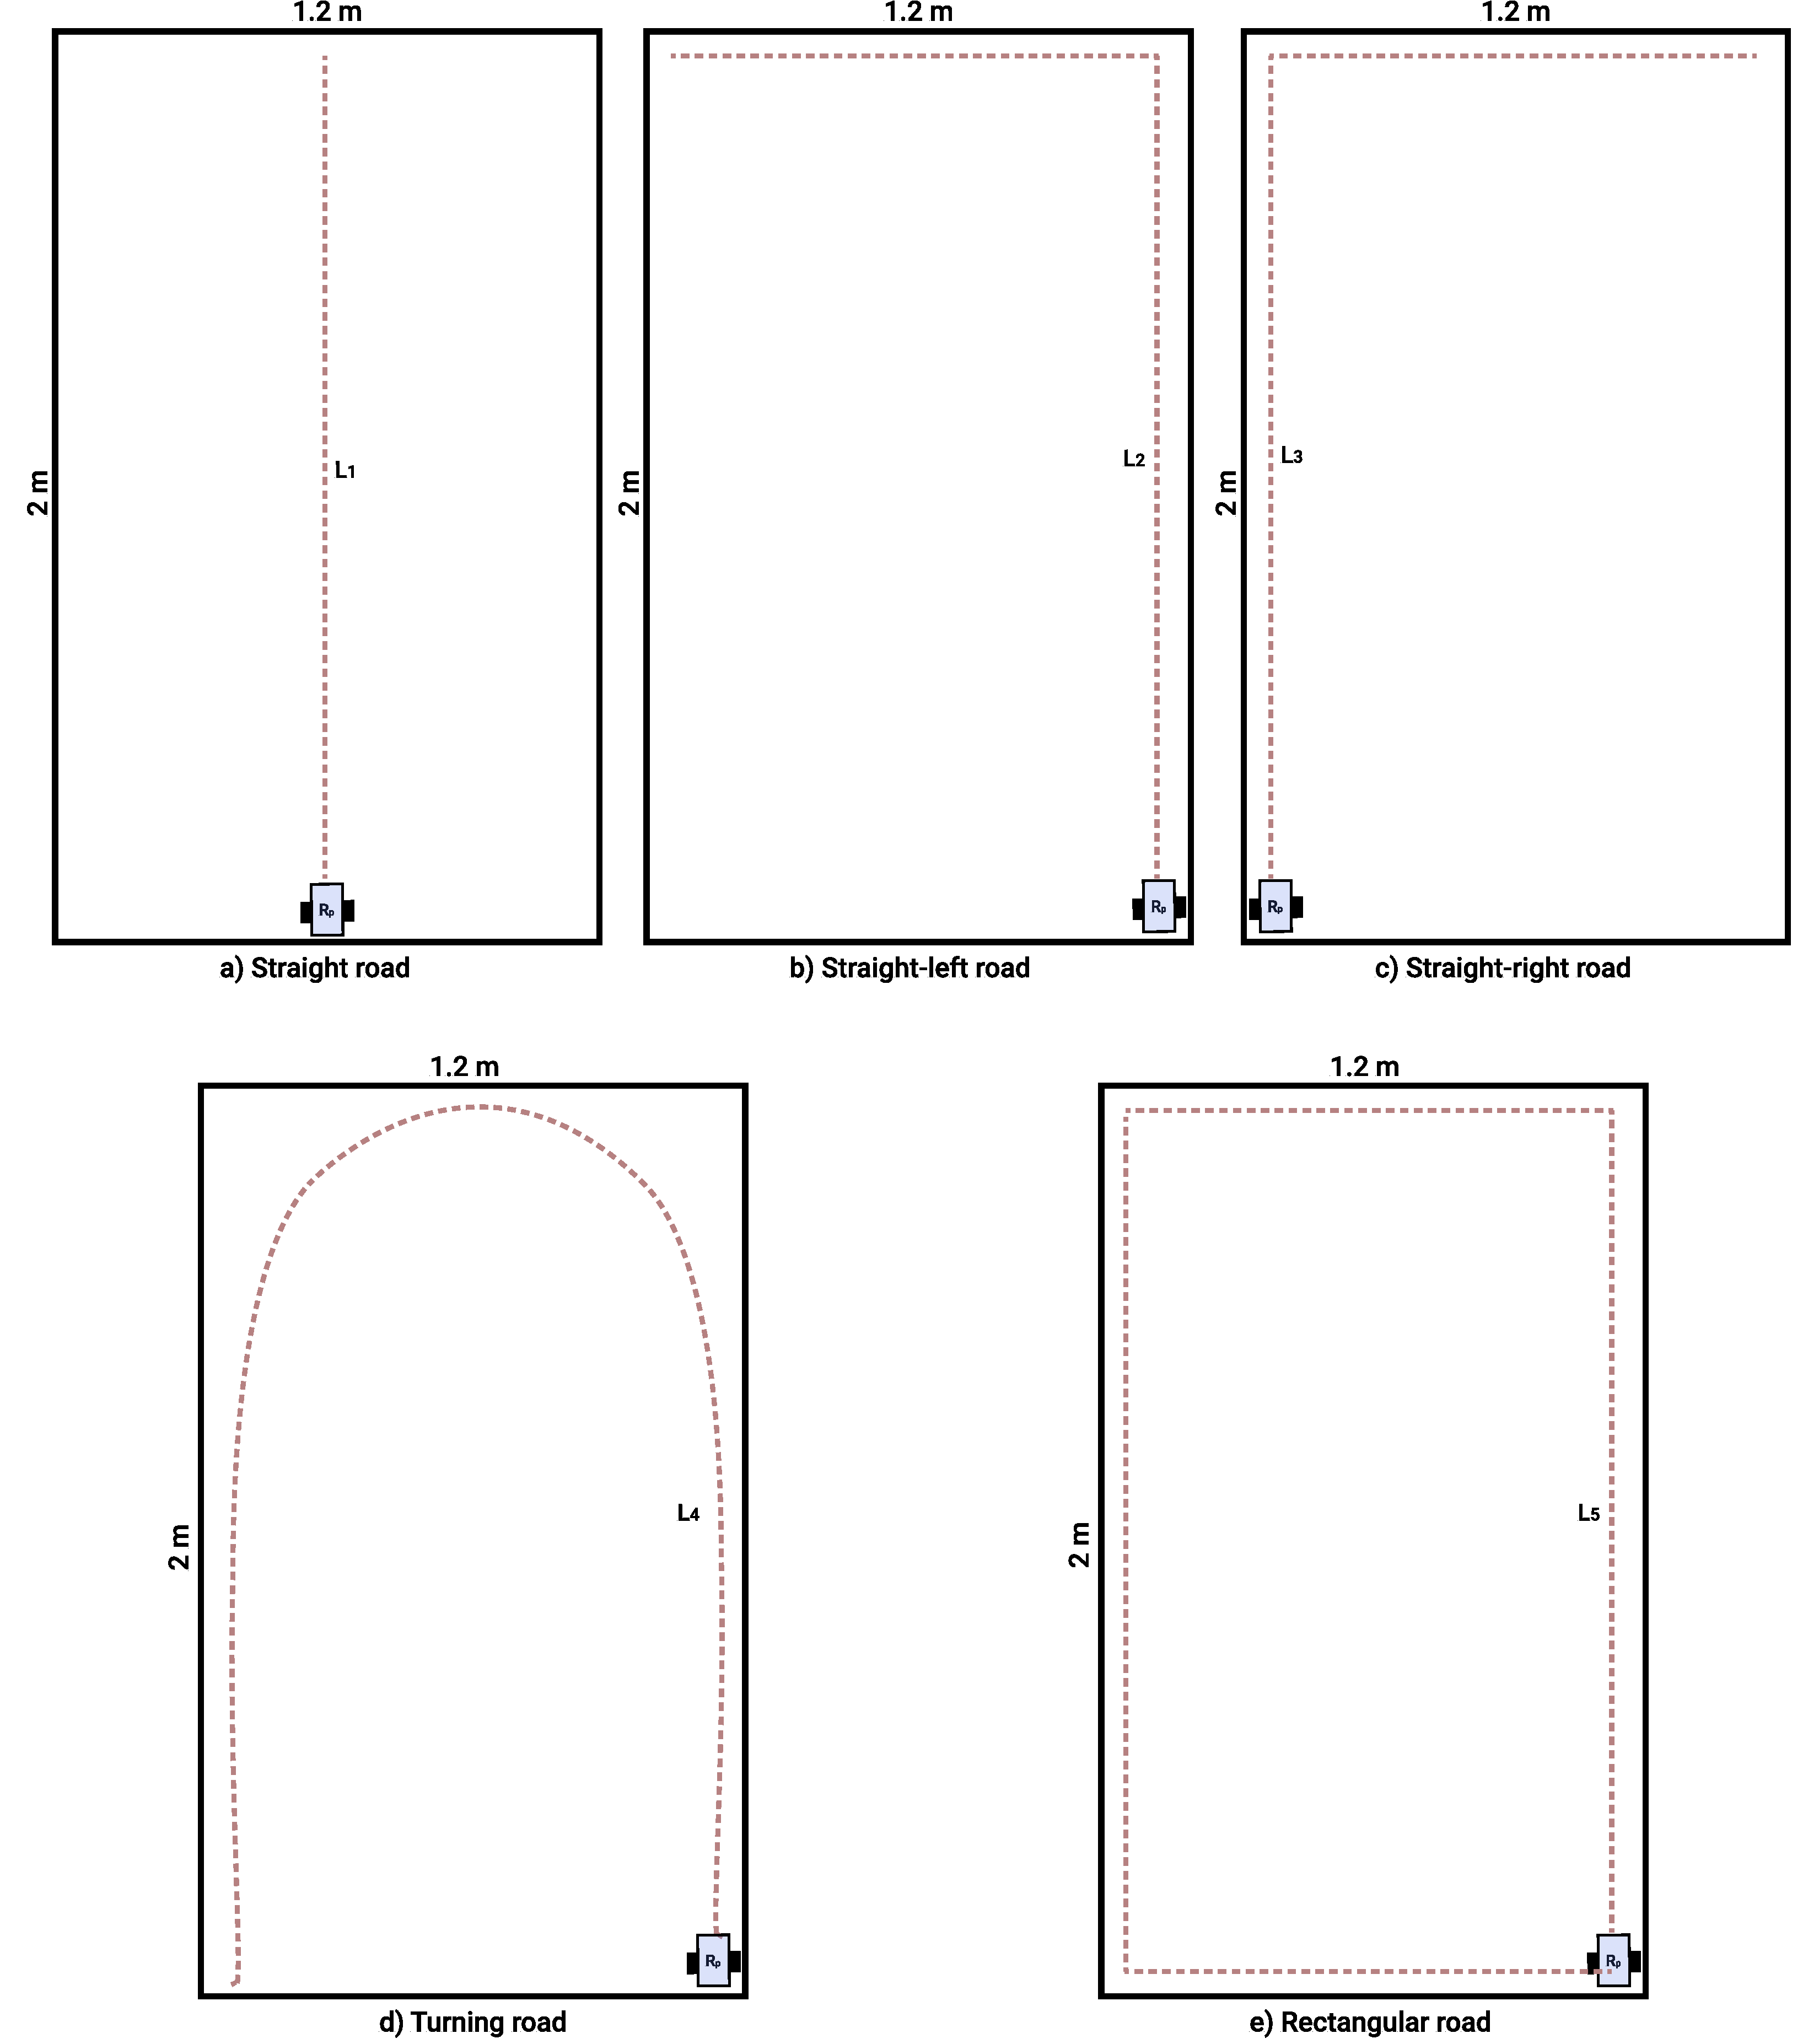
\includegraphics[width=.99\textwidth,angle=0]{figure 4-2+.pdf}
    \caption{Ilustrované cesty, použitie na testovanie.}
    \label{o:411}
\end{figure}
\subsection{Detekcia značiek}
V tejto simulácii bola veľkosť značky Aruco 6 x 6 mm. 
Na detekciu značiek v obraze použite štandardne algoritmy na rozpoznávanie značiek ArUco v OpenCV so štandardnými parametrami.
 
\begin{figure}[ht!]
    \centering
    \includegraphics[width=.90\textwidth,angle=0]{figure 4-1.pdf}
    \caption{Závislosť vplyvu veľkosti oblasti značky na chybe pri zisťovaní jej polohy.}
    \label{o:41}
\end{figure} 
\vspace{3mm}

\justifying
\noindent
Uvádzame dva príklady výsledkov získaných modelovaním. 
Jedným z dôležitých parametrov, ktoré môžu byť zaujímavé pri konštrukcii meracích systémov s referenčnými značkami,
 je presnosť zistenia ich polohy v priestore, a to v uhloch náklonu aj vo vzdialenosti. Závislosť vplyvu oblasti značky
  na chybu ovplyvňujúcu jej polohu získanú pri modelovaní je uvedená na obr. 4-1. Závislosti ukazujú, že zmenšenie 
  veľkosti značky na obrázku vedie k zvýšeniu chyby.
\vspace{3mm}
 
\justifying
\noindent
Obrázok 4-2 zobrazuje pravdepodobnosť nájdenia značky v závislosti od jej oblasti na obrázku pre
3 rôzne uhly naklonenia: 0, 45, 70. Zo závislosti je zrejmé, že značka
pravdepodobnosť rozpoznania pre uhol náklonu 0 ° sa výrazne líši od 100 v dvoch oblastiach:
s plochou 300 pixelov a s plochou v rozsahu 350-450 pixelov. Tento výsledok je
dôsledne opakované pre rôzne série modelovania s rôznymi počiatočnými parametrami.
Navyše pre značky s niekoľkými číslami v slovníku druhá oblasť (oblasť v rozsahu 350-450 pixelov) zmizne. Vysvetlenie tohto správania je jedna z úloh pre ďalšiu prácu.
\begin{figure}[ht!]
    \centering 
    \includegraphics[width=.90\textwidth,angle=0]{figure 4-2.pdf}
    \caption{Pravdepodobnosť detekcie značky v závislosti od jej oblasti na obrázku pre 3 rôzne uhly naklonenia: 0°, 45°, 70°.}
    \label{o:42}
\end{figure}

\subsection{Navigácia pre systém viacerých robotov}
V tejto časti sa najskôr simuláciou sleduje správanie robota vzhľadom na jeho dynamický pohyb cieľa. 
Ďalej sa vykoná experiment s tromi robotmi na dosiahnutie a udržanie trojuholníkového útvaru.
\subsubsection{Variácia uhlovej rýchlosti virtuálnej štruktúry}
Táto časť ukazuje dôležitosť ohraničenia uhlovej rýchlosti virtuálnej štruktúry $ \theta $ 
podľa kinematických obmedzení robotov. Preto sa simuluje mobilný robot, ktorý dosiahne virtuálny cieľ. Maximálna uhlová rýchlosť robota je $ \omega_{max} = 3./s$. Vyberieme $k = 0,6s^{-1})$.
\begin{figure}[ht!] 
    \centering
    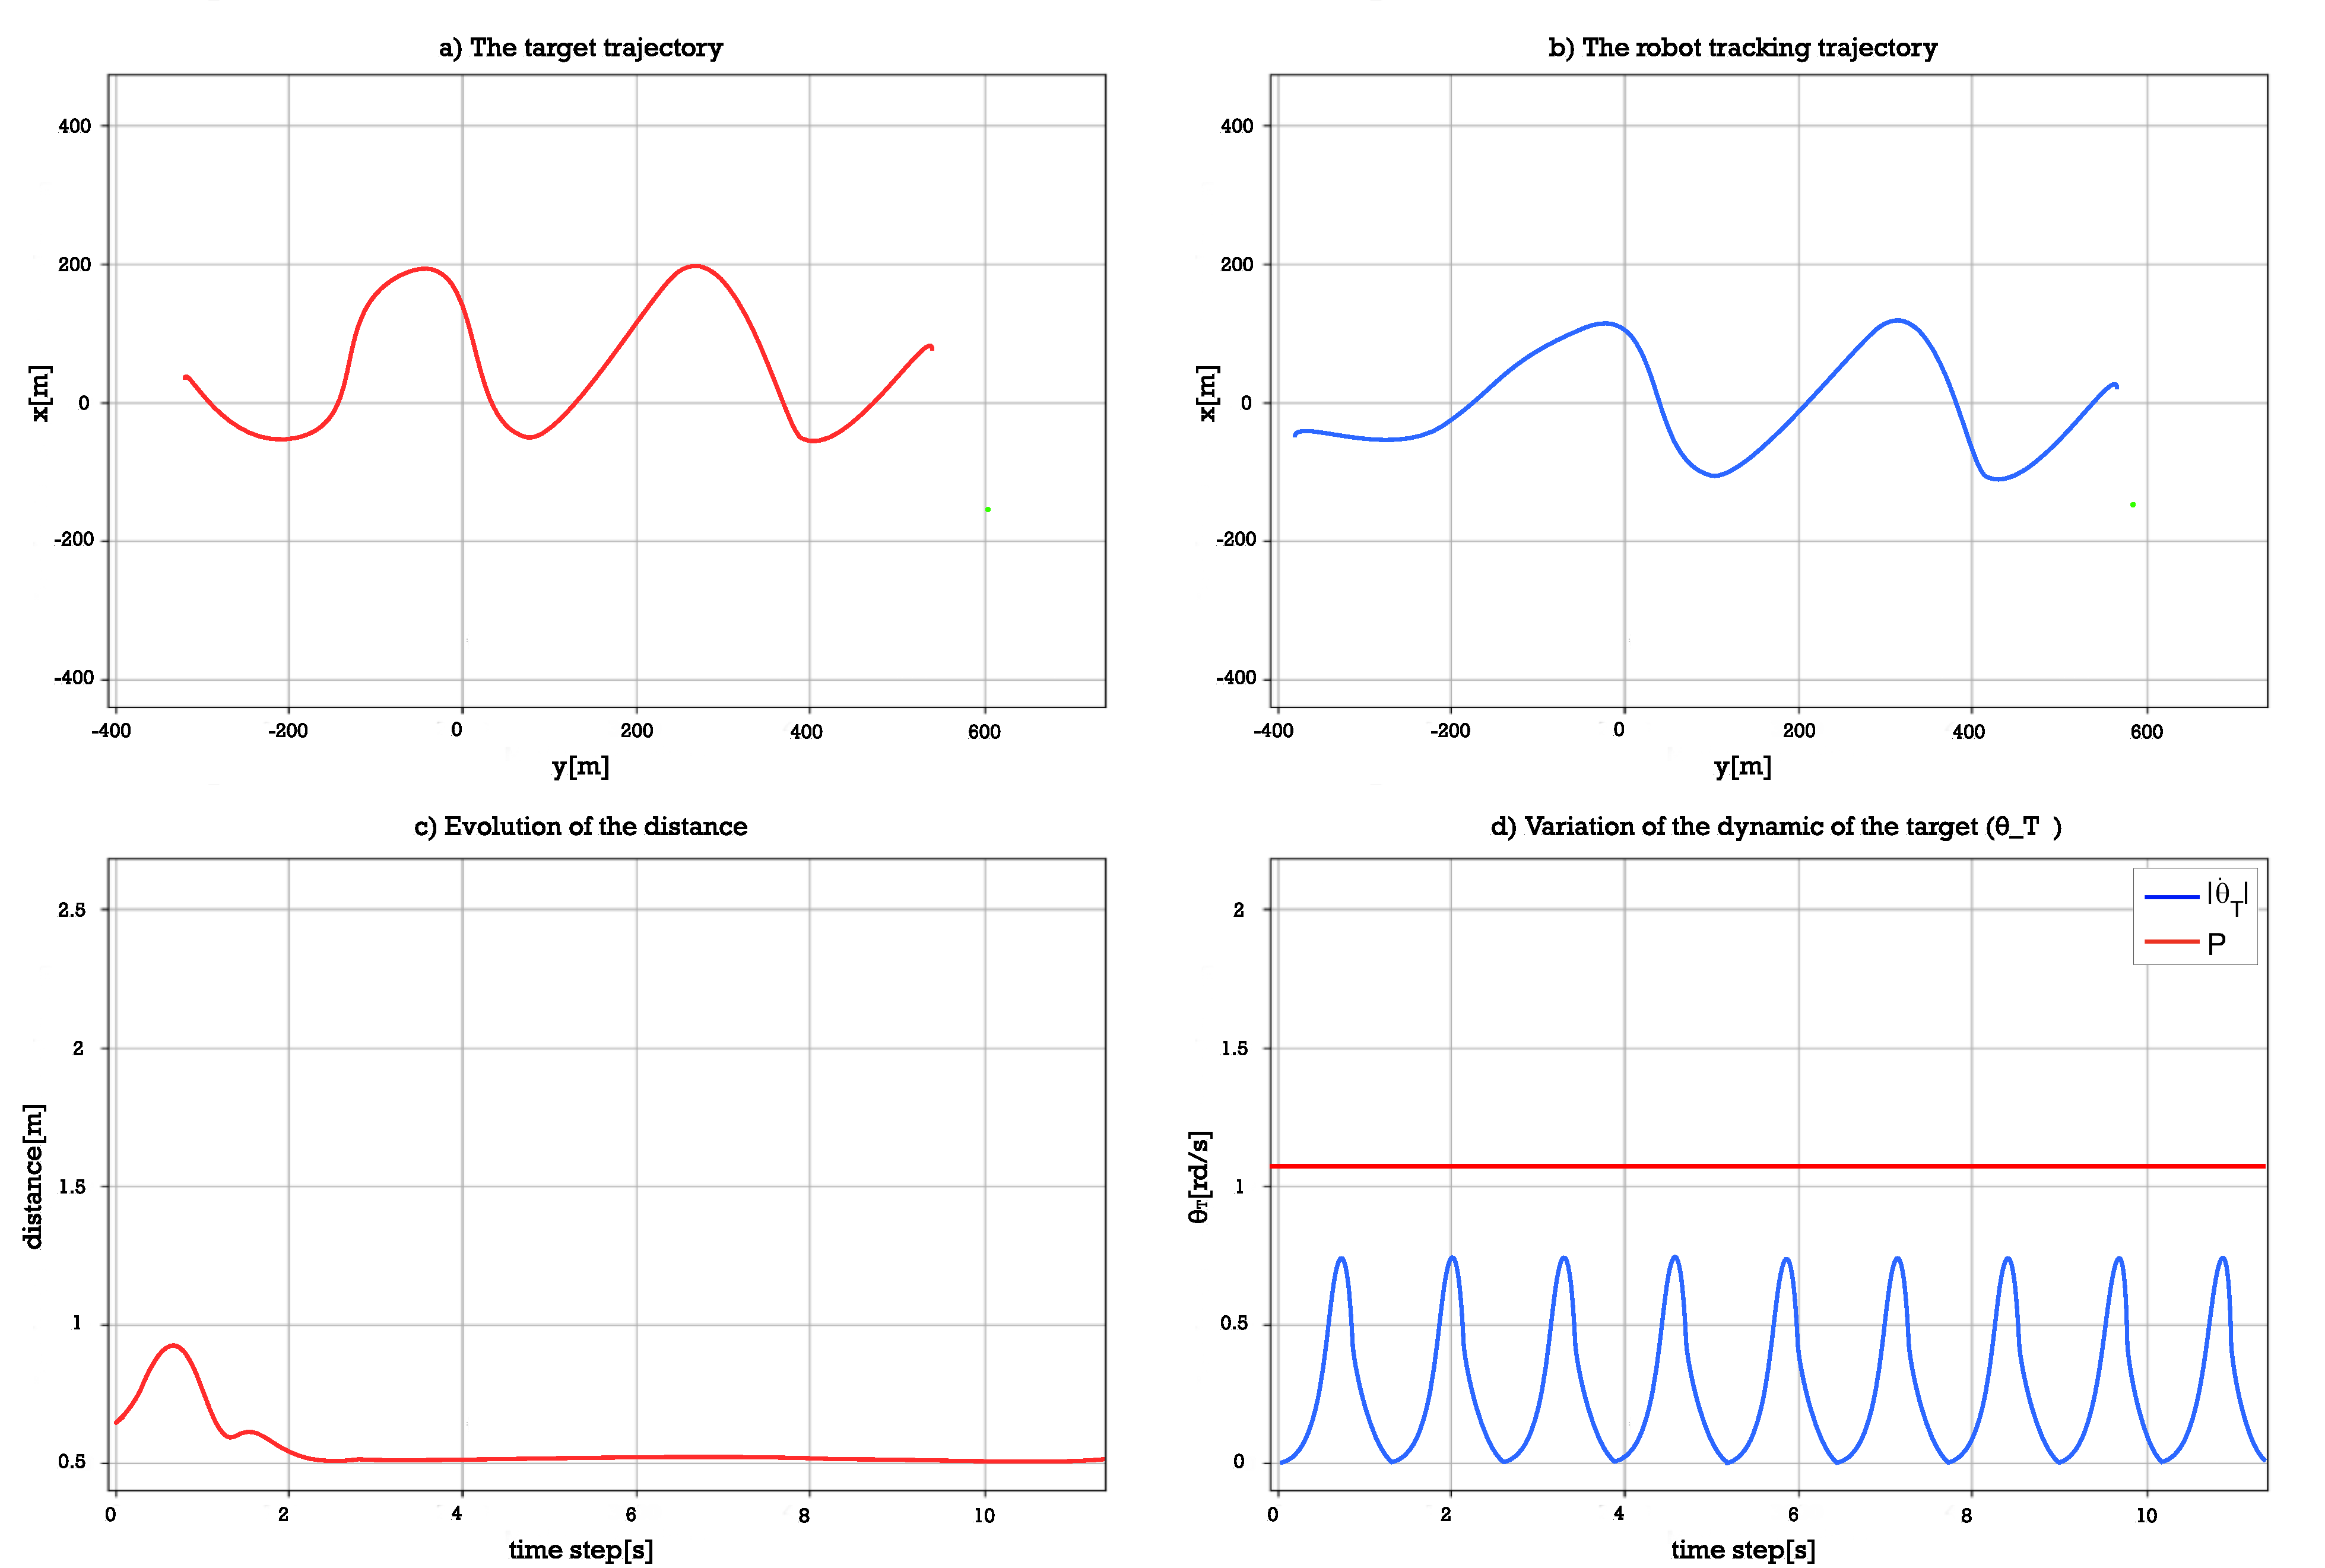
\includegraphics[width=.90\textwidth,angle=0]{figure 4-3.pdf}
    \caption{Nie sú vynútené nežiaduce kmity dráhy robota prechodnej fázy.}
    \label{o:43}
\end{figure}
\vspace{3mm}

\justifying
\noindent 
Podľa vzťahu a kvôli zjednodušeniu zápisu na číslach navrhujeme zaznamenať $ P = \omega_{max} - k \pi $. 
Na základe zvolených hodnôt $ \omega_{max} $ a $ k $ nájdeme P = 1,1. Najskôr sa navrhuje ukázať dôležitosť prechodnej fázy, 
pri ktorej musí byť variácia $ \theta_T $ nastavená na 0.
Preto teda na obrázku 4-4(d) vidíme, že $\theta_T$ sa zvyšuje na začiatku simulácie (od 0,1 s) a cieľová trajektória nasleduje okamžite po významnej krivke (porovnajte obrázok 4-4(a-b)). Následne sledujeme oscilácie na trajektórii robota. Robot správne dosiahne cieľ iba v prípade, že tento má priamu trajektóriu ($\theta_T$ = 0). Obrázok 4-4(d) to potvrdzuje. V skutočnosti, aj keď $\theta_T$ uspokojí podmienku opísanú v rovnici 
\begin{gather}\label{r:2}
    |\theta_T| \leq \omega_{max} - k\pi
\end{gather} 
, môžu sa objaviť oscilácie, ak nie je zavedená prechodná fáza. Prirodzene, že vzdialenosť $d_S$ v tomto prípade osciluje (porovnajte obrázok 4-4(c)).
\vspace{3mm}

\justifying
\noindent 
Obrázok 4-5 zobrazuje dôležitosť splnenia stavu opísaného vo vzťahu 4.1 po prechodnej fáze. Akonáhle je cieľ dosiahnutý ($\theta_T$ = 0 do okamihu 0,5 s), je splnená aj podmienka 4.1. Vidíme, že robot ide smerom k cieľu. Aj keď sa zvyšuje, variácia P je taká, že $\theta_T$ < P (porovnajte obrázok 4-5(d)). V tomto intervale robot správne sleduje svoj cieľ (porovnajte obrázok 4-5(a-b)). Vzdialenosť $d_{S_i}$, ktorá ich oddeľuje, je $d_{S_i}$ = 0 (porovnajte obrázok 4-5(c)). Po 9,5 s odstránime obmedzenie (4.1) tak, že $\theta_T$ môže byť $\theta_T$ > P. Vidíme, že robot nemôže sledovať cieľ.
\begin{figure}[ht!]
    \centering
    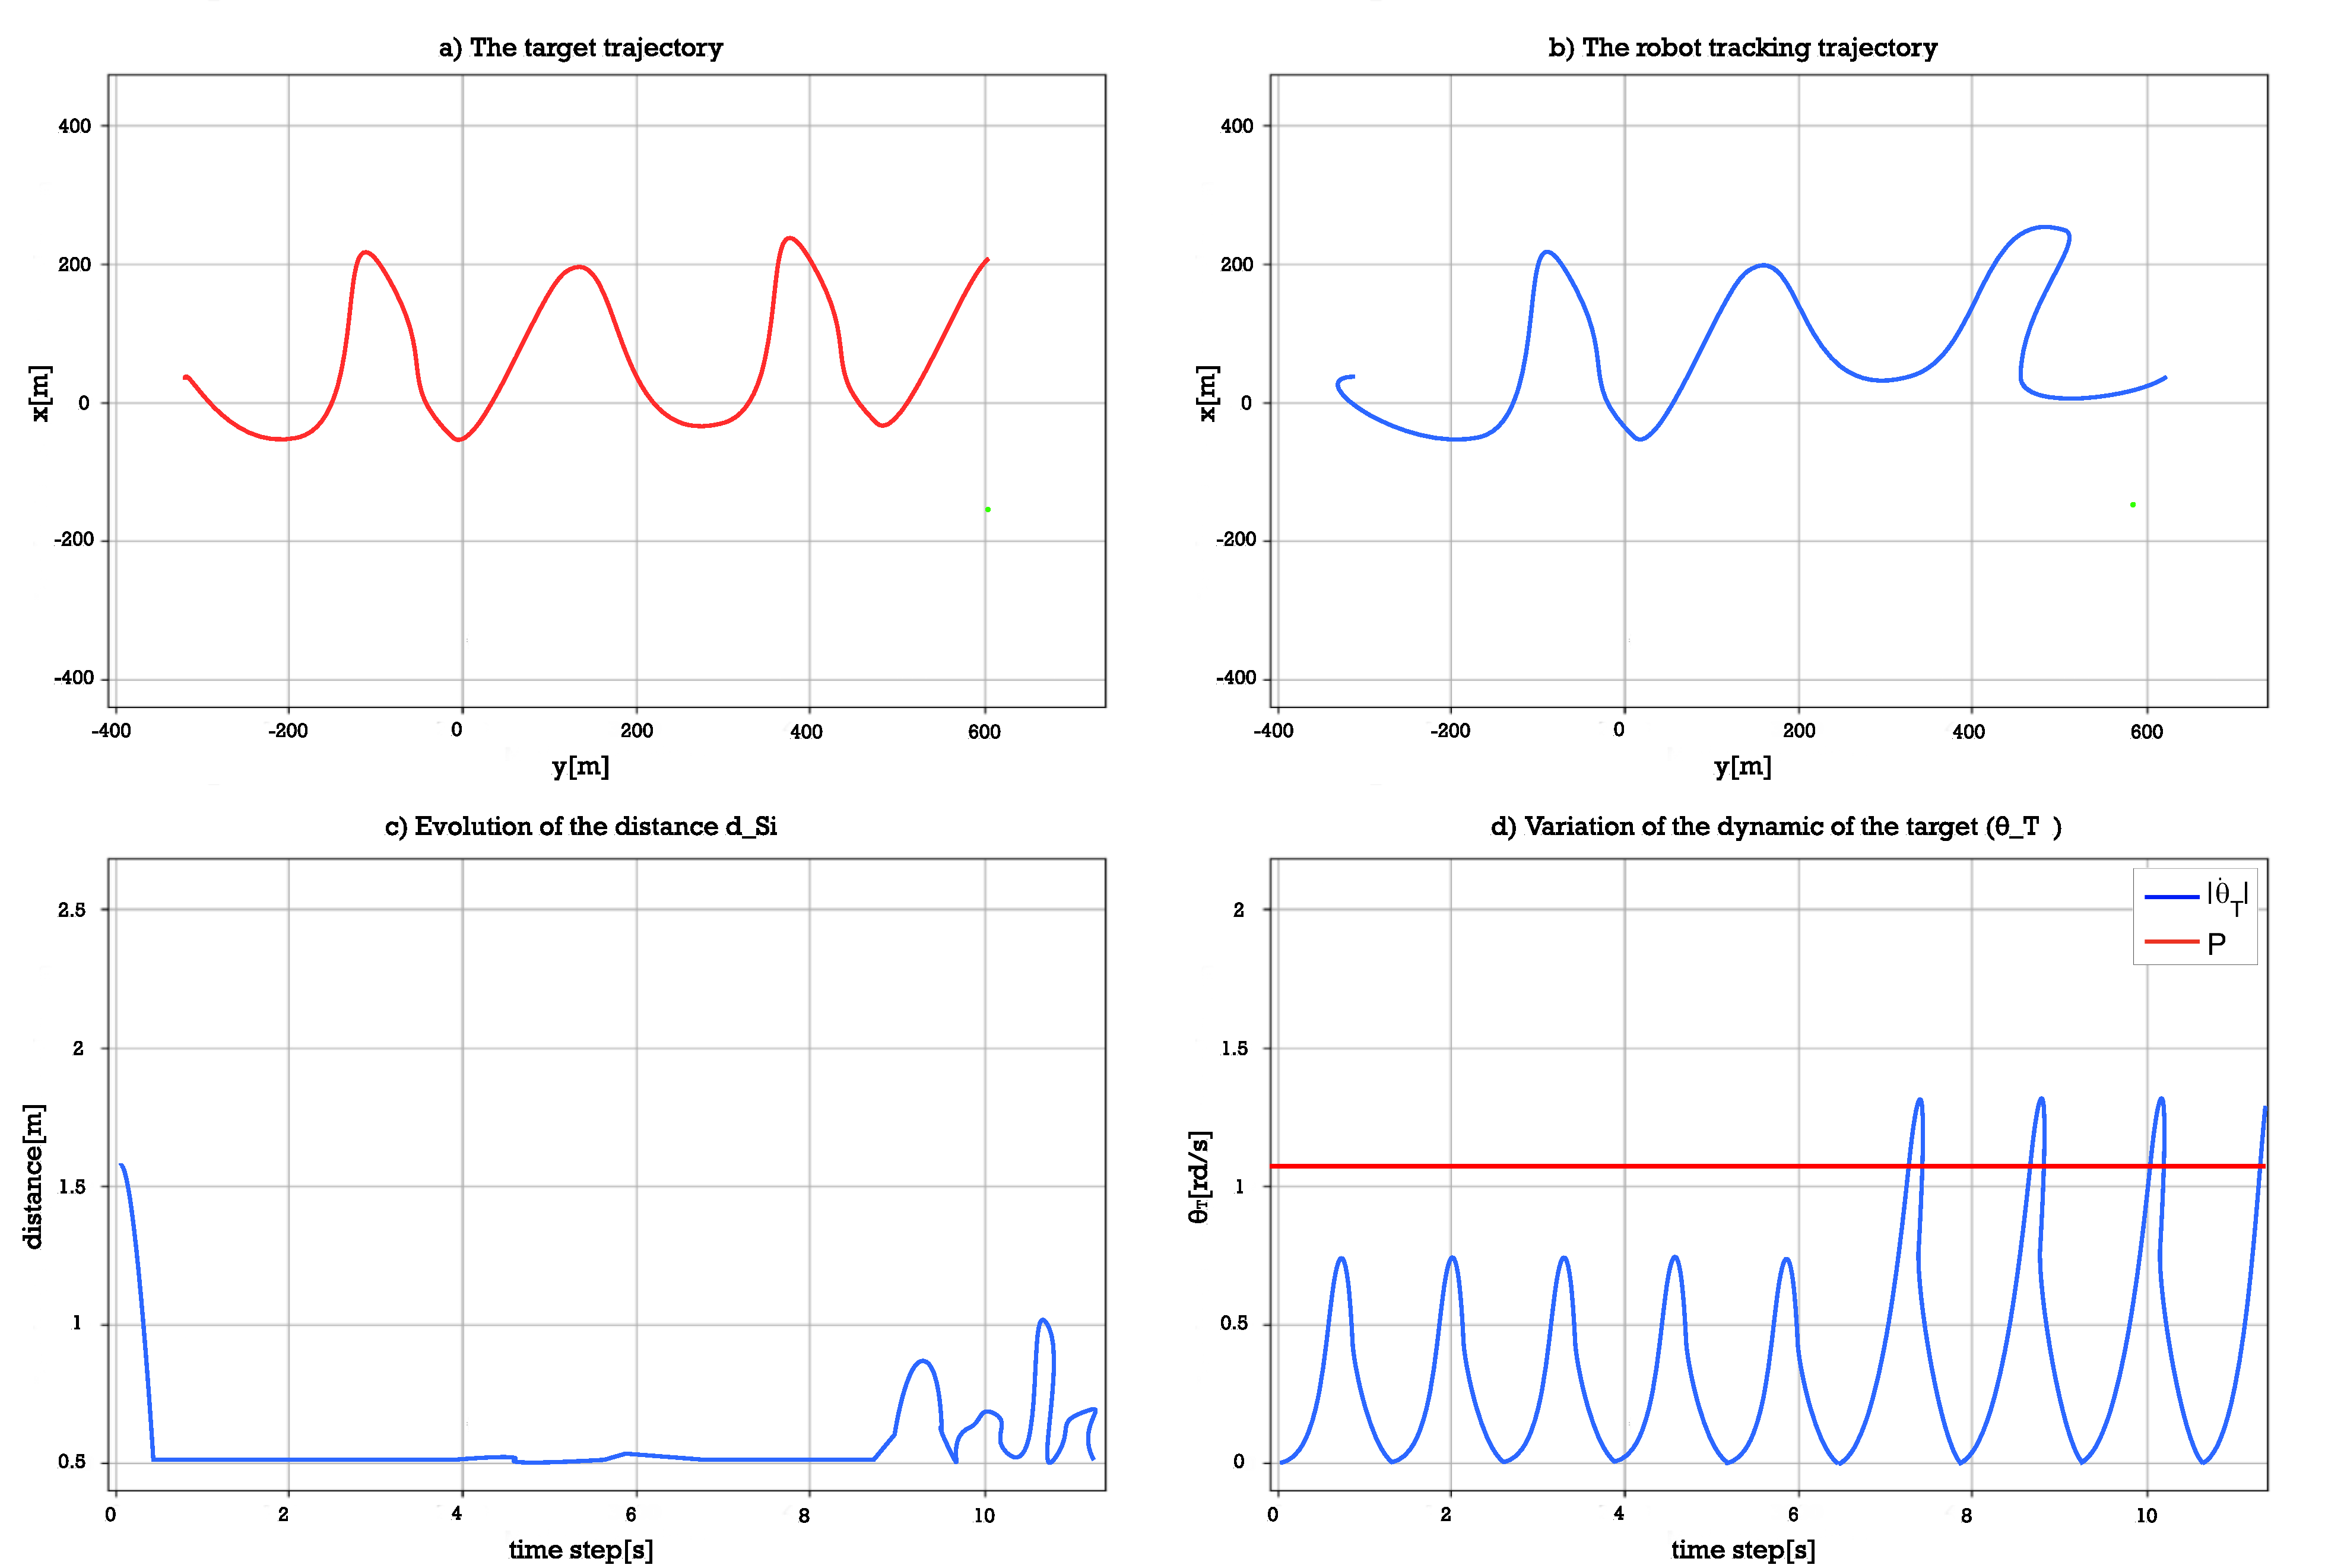
\includegraphics[width=.90\textwidth,angle=0]{figure 4-3sec.pdf}
    \caption{Nežiaduce oscilácie dráhy robota, ak nie sú splnené predpokladané obmedzenia dynamického cieľa (ak $\theta_T > P$).}
    \label{o:44}
\end{figure}

\subsubsection{Výsledky experimentu: 3 roboty s dosiahnuteľnou virtuálnou štruktúrou }
Pre tento experiment boli použité 3 roboty. Každý z nich vie o polohe a orientácii ostatných, tieto informácie boli zhromaždené pomocou odometrie. Pre tento experiment bol použitý centralizovaný systém. Experimentom je pohyb robotov v kruhu v smere hodinových ručičiek.
\vspace{3mm}

\justifying
\noindent 
Virtuálna štruktúra má priamu trajektóriu. Tu sa navrhuje rozšíriť na kruhový pohyb tak, aby všetky ciele napriek ich kinematickým obmedzeniam zostali dosiahnuteľné všetkými robotmi. S vedomím, že dynamika virtuálnej štruktúry musí sledovať vzťah, bol polomer $R_{vs}$ kruhového pohybu formovaný ako:
\begin{gather}\label{r:5}
    R_{vs} = \frac{v_T}{\theta_T} > \frac{v_T}{\omega_{max} - k \pi};
\end{gather}
kde $v_T$ je konštanta a $v_T \ll v_{max}$


\justifying
\noindent 
Uvažujeme o pohybe v smere hodinových ručičiek(obrázok 4-6)
\begin{figure}[ht!]
    \centering
    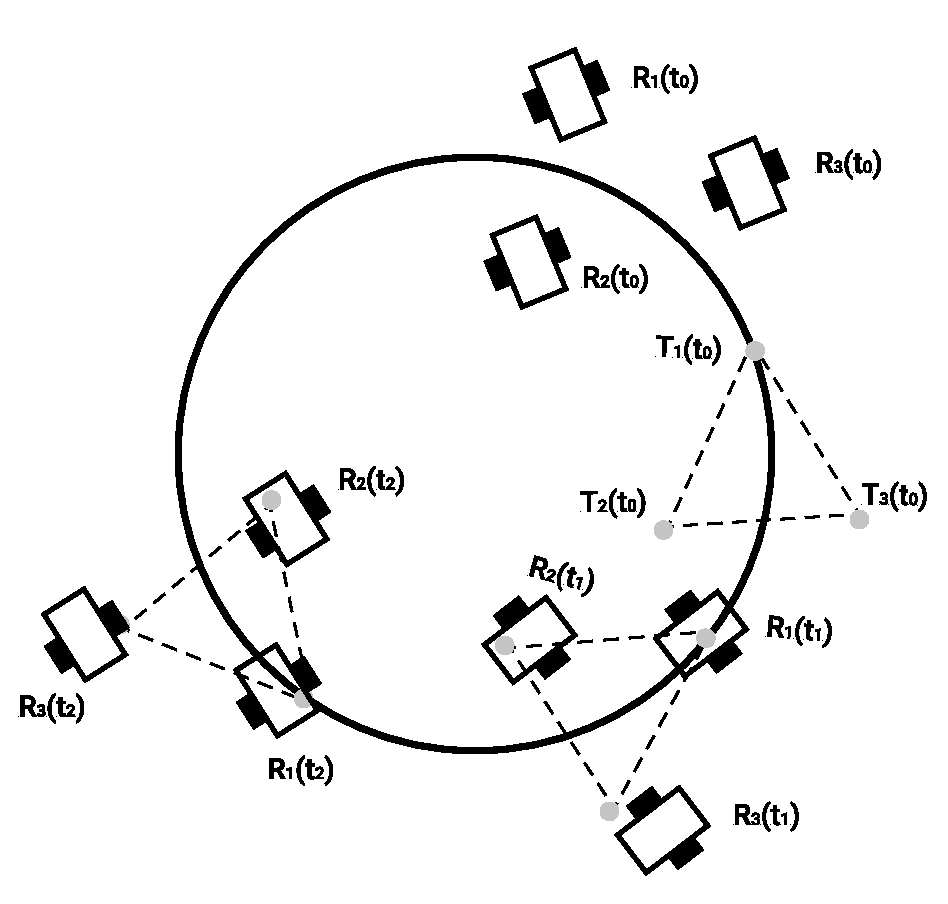
\includegraphics[width=.60\textwidth,angle=0]{figure 4-4.pdf}
    \caption{Trajektória robotov.}
    \label{o:44}
\end{figure}

\justifying
\noindent 
Ako vidíme na obrázku 4-6, skupina robotov začala v polohe udalosti do požadovanej polohy, ale nie v správnej orientácii. Ako východiskový bod experimentu si vezmeme bod $T$, v ktorom už roboty vytvárajú požadovanú štruktúru. Ako vidíme v čase $t_1$, ktorý je prvým kontrolným bodom, práce takmer sledujú ideálnu štruktúru,
ale stále existujú menšie chyby. Spájam to s nedokonalým výkonom snímača a nedokonalou komunikáciou. Na nasledujúcom kontrolnom bode, v čase $t_2$, vidíme o niečo lepší obraz o dodržiavaní ideálnej štruktúry, ale stále s malými chybami. Ak to vezmeme ako celok, môžeme s istotou povedať, že skupina robotov sa pri pohybe v kruhu drží štruktúry, a drobné chyby je nevýznamný pri plnení požadovaného typu úlohy, a to prenasledovania koristi. Vzdialenosti medzi robotmi a ich cieľmi sú uvedené na obrázku 4-7. Zmenšili sa oni do 0, čo potvrdzuje, že tvar bol dosiahnutý a udržiavaný. Keď sa zmenila dynamika virtuálnej štruktúry, roboty boli ďaleko od svojich cieľov, čo vysvetľuje pozorované skoky.
\begin{figure}[ht!]
    \centering
    \includegraphics[width=.99\textwidth,angle=0]{figure_4-8.pdf}
    \caption{Zmena vzdialenosti $d_{S_i}$ medzi robotom i a zvoleným cieľom (i = 1..3).}
    \label{o:44}
\end{figure}

\subsection{Proces prenasledovania} 
Táto časť používa na simuláciu v experimentoch grafické rozhranie Rqt a RVIZ. V oblasti štvorca 100m * 100m nie je žiadna prekážka. Modrá bodka je v mene poľovníckeho robota, červená hviezda predstavuje cieľového robota, ako je to znázornené na obrázku 4-8(a). Počiatočné polohy poľovníckych robotov a cieľového robota sú náhodne rozložené v rámci štvorcovej oblasti, čo viac odráža platnosť simulácia. Po začiatku úlohy prenasledovania môže každý robot získať informácie o polohe všetkých robotov v prostredí v reálnom čase. Pri úspešnom dosiahnutí, roboti chytia cieľ a znemožnia mu pohyb, čo sa nazýva koniec prenasledovania.
V prvej sade experimentov sú tri roboty prenasledovateľa, ktorých počiatočné informácie o polohe sú (38, 77), (44, 73) a (52, 81). Informácie o počiatočnej polohe cieľového robota sú (40, 45), ako je znázornené na obrázku 4-8(a).
\begin{figure}[ht!]
    \centering
    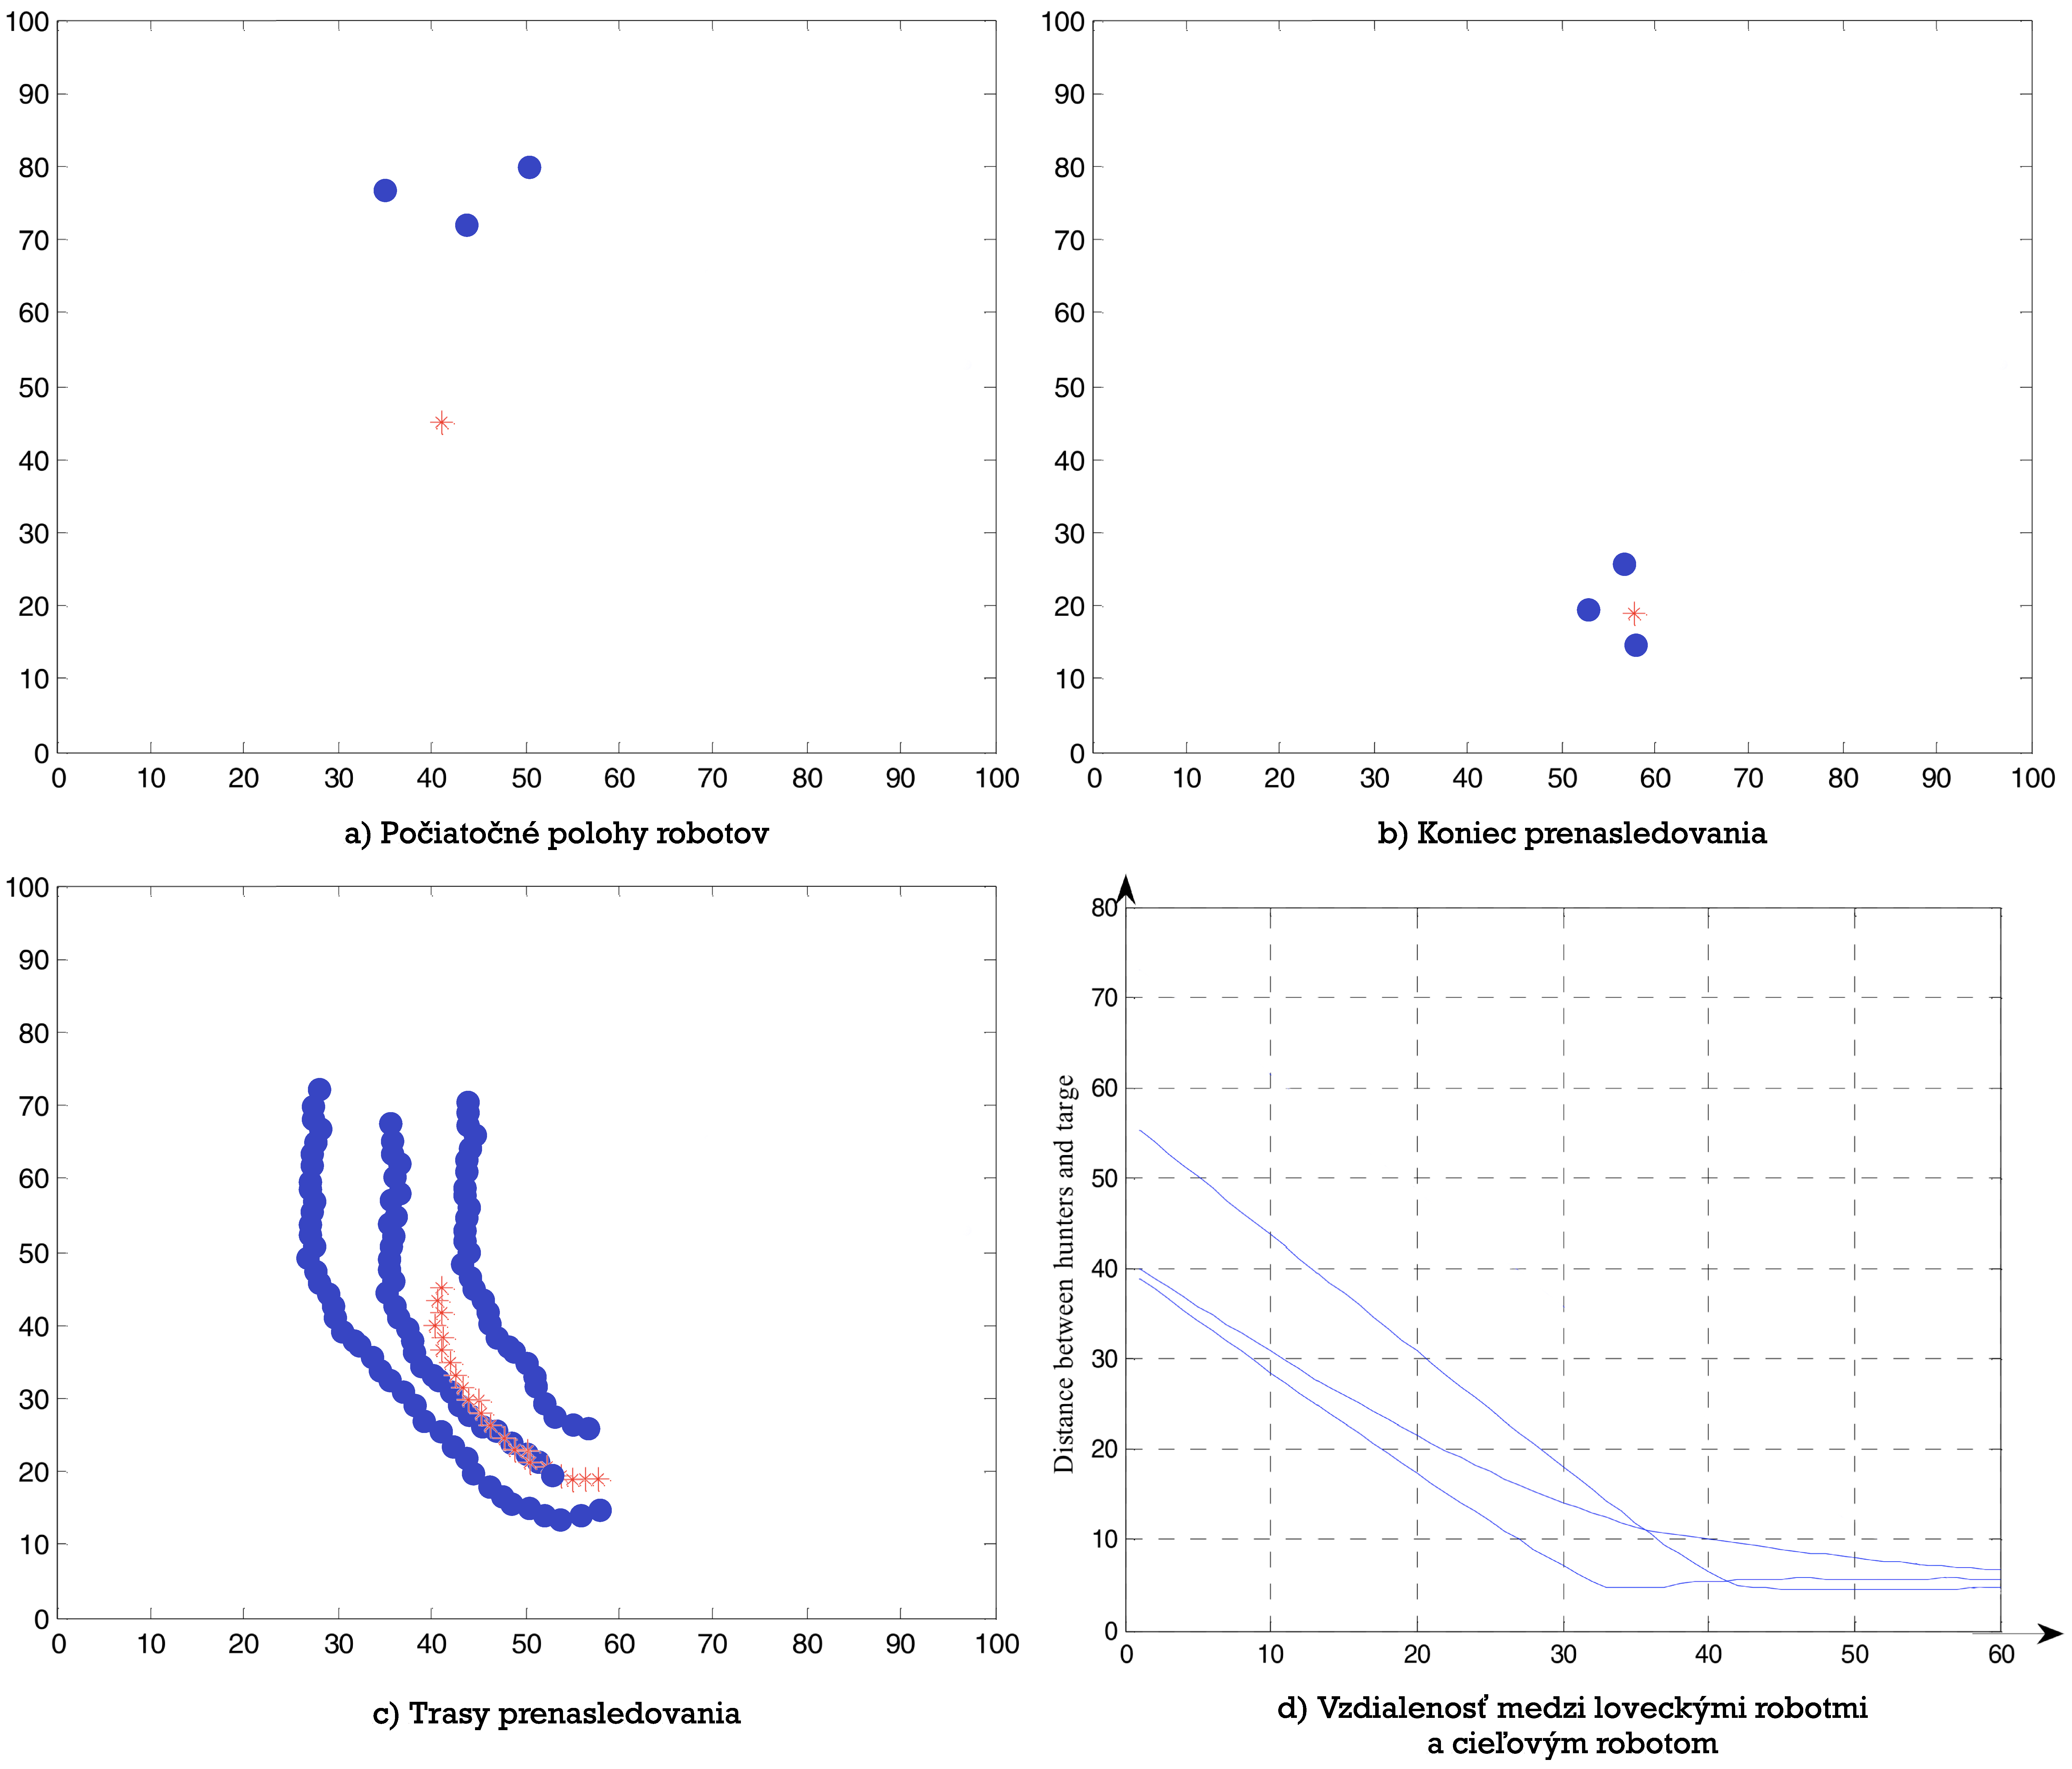
\includegraphics[width=.99\textwidth,angle=0]{figure_4-9.pdf}
    \caption{Výsledky simulácie}
    \label{o:44}
\end{figure}

\justifying 
\noindent 
Konečný výsledok prenasledovania je uvedený na obrázku 4-8(b). Tri prenasledovatelia sa rovnomerne rozložia okolo cieľového robota, aby si cieľ nemohol zvoliť ďalší pohyb, čo znamená úspešný lov. Z trajektórie procesu prenasledovania, ako je znázornené na obrázku 4-8(c), vidíme, že trajektória prenasledovacieho robota je veľmi hladká. Keď štyri prenasledovacie roboty dorazia do potrebnej oblasti, začnú upravovať svoje polohy tak, aby obkolesili cieľ. Červená krivka predstavuje trajektóriu cieľa a vidíme, že korisť tiež neustále uniká prenasledovateľov. Ako je znázornené na obrázku 4-8(d), os $X$ predstavuje počet opakovaní herného procesu, os $Y$ predstavuje vzdialenosť medzi prenasledovacím robotom a cieľom a všetky tri modré plné čiary predstavujú krivku zmeny vzdialenosti medzi tromi robotmi a cieľov resp. Ukazuje to, že roboty sa postupom času neustále približujú k cieľu. Pri hľadaní potrebnej polohy sa roboti začnú skôr pohybovať s cieľom, ako by sa mali približovať, čo dokazujú sklony kriviek plných modrých čiar. Keď posledný prenasledovací robot dosiahne svoju pozíciu, cieľ sa považuje za úspešne chytený a systém sa zastaví.
\begin{table}[h!]
    \centering
        \begin{tabular}{|c c c|} 
        \hline
        Veľkosť oblasti & Priemerný počet krokov & Úspešnosť \\ [0.5ex] 
        \hline\hline
        100m*100m & 90.26 & 78\% \\ 
        \hline
        60m*60m & 62.14 & 76\% \\
        \hline 
        40m*40m & 47.23 & 69\% \\
        \hline 
       \end{tabular}
       \caption{Výsledkom simulácie na ploche 100m * 100m vs 60m * 60m }
        \label{table:1}
\end{table}
\begin{table}[h!]
    \centering
        \begin{tabular}{|c c c|} 
        \hline
        Rýchlosť prenasledovateľov & Priemerný počet krokov & Úspešnosť \\ [0.5ex] 
        \hline\hline
        0.05 & * & 0\% \\ 
        \hline
        0.07 & 99.26 & 20\% \\
        \hline 
        0.1 & 77.48 & 100\% \\
        \hline 
        0.2 & 50.04 & 100\% \\
        \hline 
        0.4 & 34.28 & 100\% \\
        \hline 
       \end{tabular}
       \caption{Výsledky simulácie 3 prenasledovateľov v oblasti 100 m * 100 m}
        \label{table:1}
\end{table}

\justifying 
\noindent 
Tabuľka 4-2 zobrazuje priemerný počet krokov a úspešnosť v loveckej úlohe s podmienkou vyššej rýchlosti prenasledovateľov a náhodným generovaním informácií o ich polohe. Ako je uvedené v tabuľke, pri veľkosti oblasti 100 m x 100 m bude úspešnosť 78\%. Medzitým je priemerný počet krokov k lovu 90,26 krokov. Pre ďalší variant bol experimentálny priestor zmenený na plochu 60m * 60m. Miesta loveckých robotov sú generované náhodne a maximálna rýchlosť loveckých robotov je stále vyššia ako cieľový robot. V súčasnosti majú tieto tri lovy takmer rovnakú úspešnosť ako v predchádzajúcej oblasti, ale priemerný počet krokov je znížený na 62,14 krokov. Teda údaje v tabuľke 4-2 ukazujú, že počiatočné polohy prenasledujúcich robotov majú vplyv na poľovnícku úlohu. 
Tabuľka 4-3 ukazuje výsledky loveckých experimentov, v ktorých traja roboti prenasledovatelia náhodne vygenerovaní v oblasti 100 m * 100 m a pri rôznych rýchlostiach dokončili 20 experimentov. Ako ukazuje tabuľka, pri rýchlosti 0,05 m/krok, ktorá je rovnaká ako u robota koristi, nie je lovecký robot schopný dokončiť úlohu. Keď sa rýchlosť prenasledovateľov zvýši o 0,02 m/krok, úspešnosť lovu sa zvýši tiež na 20\% a priemerný počet krokov k úspešnému lovu je 99 krokov. Keď sa rýchlosť zvýši na 0,1 m/krok, úspešnosť je až 100\% a priemerný počet krokov je 77,48 kroku. Ak sa rýchlosť zvýši na 0,2 m/krok a 0,4 m/krok, priemerný počet krokov sa zodpovedne zníži. Ukazuje, že relatívna rýchlosť medzi loveckými robotmi a cieľovým robotom je veľmi znepokojujúca z hľadiska efektívnosti kooperatívneho prenasledovania s viacerými robotmi v tabuľke 4-3.
\vspace{3mm}

\justifying
\noindent 
Stručne povedané, navrhovaný algoritmus môže efektívne dokončiť úlohy prenasledovania s viacerými robotmi. Pri úlohe kooperatívneho prenasledovania s viacerými robotmi sú dôležitými faktormi je počet prenasledujúcich robotov, počiatočná poloha robotov a maximálna rýchlosť robotov. Keď je počet prenasledujúcich robotov veľký a ich polohy sú bližšie k robotu Koristi a robot prenasledovateľ je rýchlejší ako robot Korisť, bude úloha dokončená ešte lepšie. 

    

% V tomto experimente vyhodnocuje trajektória a vzdialenosť medzi korisťou a vyšetrovateľmi po jednom, vedúcom robotovi zo skupiny. Pohyb samotnej skupiny bol testovaný v predchádzajúcej časti. V tomto scenári sa cieľový robot pohybuje po lineárnej trajektórii. Najskôr som simuloval situáciu, keď je prenasledovateľ cieľ plne vnímaný. Výsledné správanie pri sledovaní je znázornené na obr. 2. V počiatočnej fáze (znázornenej na obr. 2a) bol prenasledovateľ ďaleko od cieľa, rýchlo akceleroval (pozrite zmenu rýchlosti na obr. 2c) smerom k cieľu a ukazoval prenasledovanie správania. V tejto fáze sa vzdialenosť medzi prenasledovateľom a cieľom rýchlo skrátila (pozrite zmenu vzdialenosti na obr. 2c). Keď sa vzdialenosť znížila na určitú mieru, rýchlosť prenasledovateľa sa začala rýchlo znižovať, aby zodpovedala rýchlosti koristi (tj. Prvý prudký pokles rýchlosti na obr. 2c). Rýchlosť nakoniec kolísala okolo cieľovej rýchlosti, následne vzdialenosť medzi prenasledovateľom a korisťou zostávajúcou okolo r (r = 3 m).
% Celá trajektória prenasledovateľa je udržiavaná blízko trajektórie cieľa, čo demonštruje koherentné sledovanie (obr. 2b). Toto je potvrdené na obrázku 2c, kde vzdialenosť medzi prenasledovateľom a cieľom konverguje do malého rozsahu, čo naznačuje, že poloha prenasledovateľa sa zbieha do susedstva s miestom umiestnenia cieľa. Upozorňujeme, že trajektória prenasledovateľa je plynulejšia ako trajektória cieľa, čo naznačuje efekt úspory energie dosiahnutý touto schémou sledovania. 
% \begin{figure}[ht!]
%     \centering
%     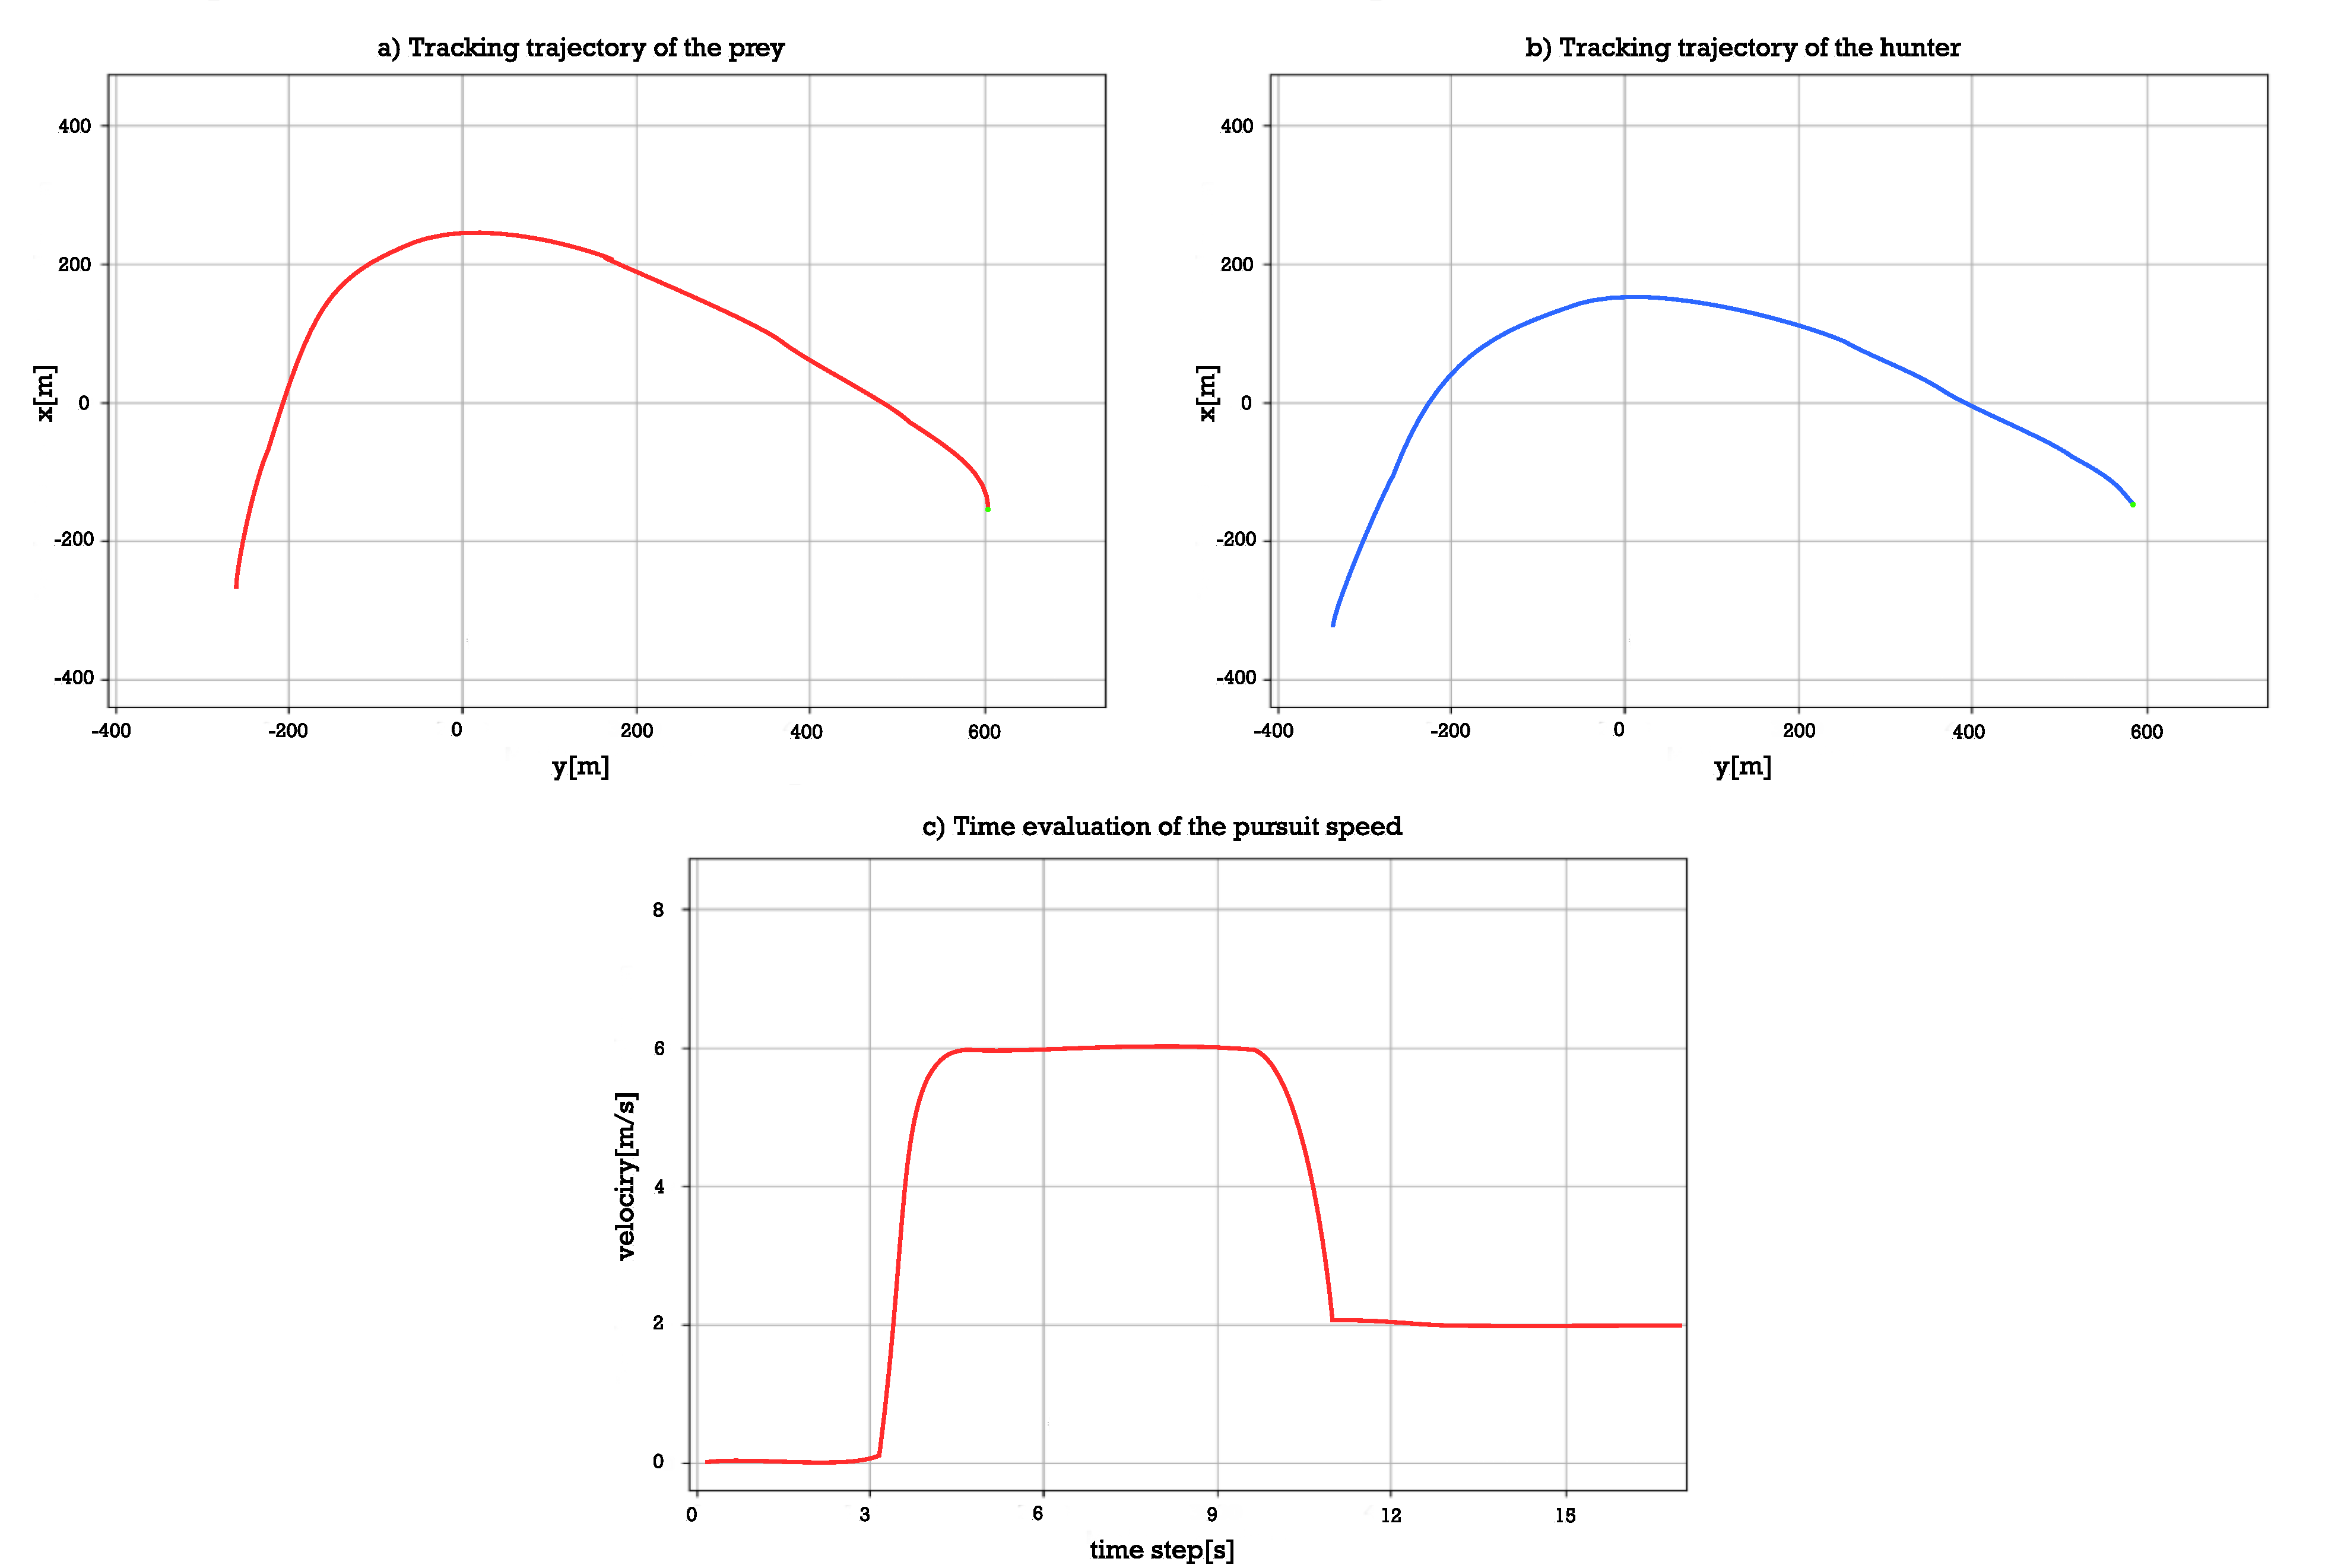
\includegraphics[width=.99\textwidth,angle=0]{figure 4-5.pdf}
%     \caption{Sledovanie korisťi.}
%     \label{o:45}
% \end{figure}